
\documentclass[english,a4paper,oneside]{ppfcmthesis}

\usepackage[utf8]{inputenc}
\usepackage[OT4]{fontenc}

% A few changes from the ppfcmthesis style

\usepackage[widespace]{fourier}                 % Use Utopia font set
\usepackage[scaled=0.875]{helvet}
\renewcommand{\ttdefault}{lmtt}

\newcommand{\customtextsc}[1]{{\scriptsize \MakeUppercase{#1}}}
\newcommand{\acro}[1]{\customtextsc{#1}}   % generic acronym

\newcommand{\pcite}[1]{[\ref{#1}]}         % product citation

\usepackage{tabularx}
\usepackage{booktabs}                                  % Booktabs for tables
\usepackage{varioref}                                  % variable references (\vref{})

% Define colors for listings.
\usepackage{xcolor}
\usepackage{listings}

\definecolor{codestrings}{rgb}{0.164,0,1}
\definecolor{codecomment}{rgb}{0.25,0.49,0.37}
\definecolor{codekeywords}{rgb}{0.49,0,0.33}
\definecolor{codebackground}{rgb}{0.95,0.95,0.95}

\lstset{
  inputencoding=utf8,
  language=Java,
  extendedchars=true,
  basicstyle=\ttfamily\scriptsize,
  numbers=left,
  numbersep=3pt,
  framexleftmargin=2pt,
  framerule=0pt,
  frame=lines,
  numberstyle=\tiny,
  tabsize=2,
  showstringspaces=false,
  showspaces=false,
  keywordstyle=\bfseries\color{codekeywords},
  identifierstyle=\color{black},
  stringstyle=\color{codestrings},
  commentstyle=\color{codecomment},
  columns=fullflexible,
  abovecaptionskip=\medskipamount,
  belowcaptionskip=\medskipamount,
  backgroundcolor=\color{codebackground},  
}

\RecustomVerbatimEnvironment{Verbatim}{Verbatim}%
    {fontsize=\footnotesize,frame=lines,numbers=left}

\lstnewenvironment{javablock}{\lstset{language=Java}}{}
\lstnewenvironment{codeblock}{\lstset{language=Java}}{}
\lstnewenvironment{rubyblock}{\lstset{language=Ruby}}{}
\lstnewenvironment{xmlblock}{\lstset{language=XML}}{}

\DefineVerbatimEnvironment{screenblock}{Verbatim}%
    {fontsize=\scriptsize,numbers=left,numbersep=3pt}

\settypeblocksize{*}{32pc}{1.618}
\setlrmargins{*}{1.47in}{*}
\setulmargins{*}{*}{1.3}
\setheadfoot{\onelineskip}{2\onelineskip}
\setheaderspaces{*}{2\onelineskip}{*}

\newcommand{\tabcaption}[1]{\multicolumn{1}{c}{#1}}
\newcommand{\code}[1]{\texttt{#1}}

\author{Marcin Zduniak}
\title{Automated GUI Testing of~Mobile~Java~Applications}
\ppsupervisor{dr inż.~Bartosz Walter}
\ppyear{2006--2007}

\begin{document}

% Front matter starts here
\frontmatter\pagestyle{empty}%
\maketitle\cleardoublepage%

% Blank info page for "karta dyplomowa"
\thispagestyle{empty}\vspace*{\fill}%
\begin{center}Tutaj przychodzi karta pracy dyplomowej;\\oryginal wstawiamy do wersji dla archiwum PP, w pozostalych kopiach wstawiamy ksero.\end{center}%
\vfill\cleardoublepage%

% Table of contents.
\pagenumbering{Roman}\pagestyle{ppfcmthesis}%
\tableofcontents* \cleardoublepage%

% Main content of your thesis starts here.
\mainmatter%

\chapter{Introduction}


\section{Overview}

Applications written for mobile devices have become more and more complex and sophisticated, adjusting to the
constantly improving computational power of hardware. With the growing application size comes the
need for automated testing frameworks, particularly frameworks for automated testing of user
interaction and graphical user interface. While such testing (also called
\emph{capture-replay}) has been thoroughly discussed in literature with respect to desktop
applications, mobile development limits the possibilities significantly. To our best knowledge only
a few solutions for creating automated tests of mobile applications exist and their functionality
is very limited in general or constrained to only proprietary devices. 
This thesis describes certain preliminary results of the attempt to design and implement a
framework for capturing and replaying user interaction in applications written for the Java 2 Micro
Edition environment. We called this prototype implementation \textsf{RobotME}.

\subsection{Mobile Application Development}

% briefly sketch the process of mobile application development in Java -- programming
% cycle (code development, obfuscation, packaging, deployment, real-device testing)

Java applications written for mobile devices (mobile phones in vast majority) are simpler and
smaller compared to their desktop or server cousins. The environment provides a simple virtual machine (JVM) for
executing the program's code and a set of generic \emph{application programming interfaces} (API)
for accessing the hardware layer -- the device's display, network or communication ports.

The development process targetting mobile applications is very similar to desktop software,
forming a loop between establishing the required feature set, planning,
actual development, software releases and maintenance. For applications featuring graphical user interface
a set of test scenarios is typically created for determining the quality and completeness of the 
produced software. A simplified illustration of relationship between development stages and testing
steps is shown in Figure~\ref{fig:process-outline-2}.

\begin{figure}[t]%
\begin{center}
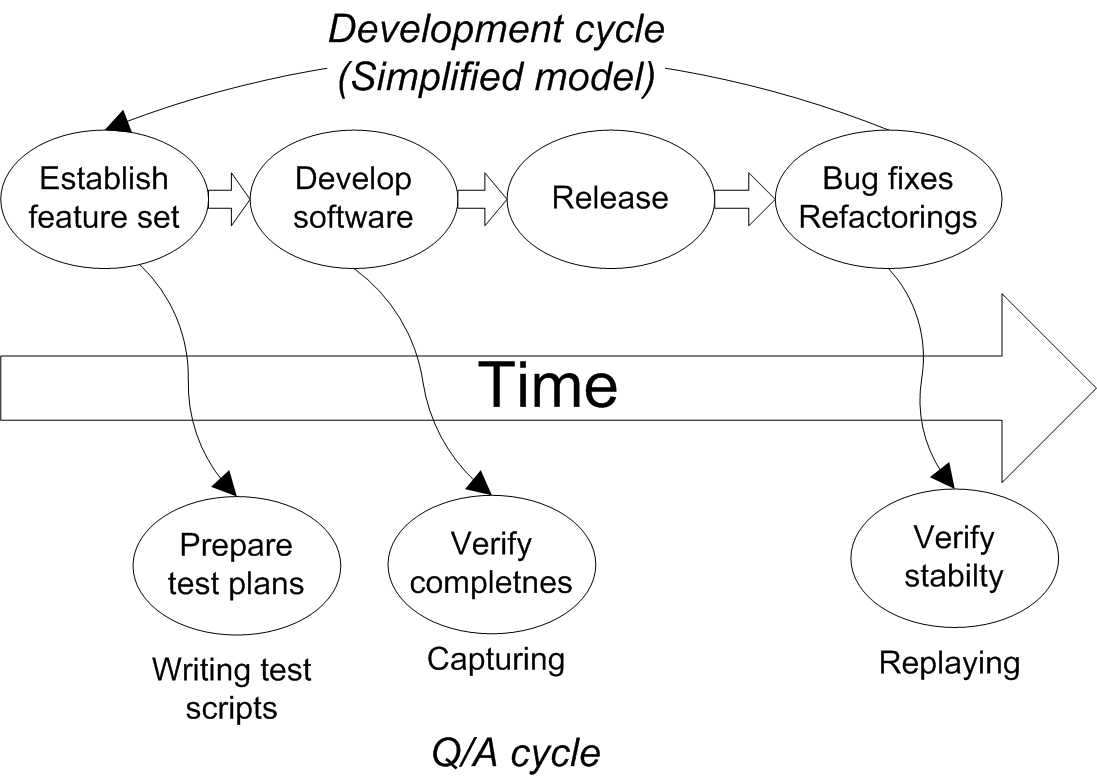
\includegraphics[width=.9\linewidth]{figures/process-outline-2}
\end{center}
\caption{Capture-replay regression test scenario in parallel to software development life cycle.}%
\label{fig:process-outline-2}
\end{figure}

In this thesis we would like to focus on the difficulties of testing mobile applications and possibilities of
automation of this process.  


\subsection{Problems of GUI Testing}

Testing mobile applications is different compared to desktop software because of several
reasons:

\begin{itemize}
    \item mobile software is written on an emulator and eventually runs on the actual device,

    \item there are less or more subtle differences between emulators and devices (and in particular across devices from different
    vendors) in terms of supported APIs, hardware and Java Virtual Machine implementation details,
    
    \item uploading and testing the application on each and every device is a tedious, time-consuming process,
    
    \item the final release of the software often differs from the development version due to obfuscation, macro expansion
    and other code-manipulation techniques.
\end{itemize}

Both programming and particularly testing are much more difficult in such an environment
compared to writing programs for the desktop. Each mobile phone, for example, has a different
hardware configuration: display size and capabilities (number of colors), size of memory and varying
computational power. Application interfaces defined by the J2ME specification and considered a
`standard', are implemented by different vendors and often contain differences that must be taken
into account, increasing the complexity of the program. The same application looks, but often also
\emph{behaves} a bit different depending on the target device it was installed on. 
The key differences between mobile and traditional software development was summarized in 
Table~\ref{tab:environments}.


\begin{table}[t]%
\caption{Differences between development and testing of mobile and traditional (desktop and server) applications.}%
\label{tab:environments}
\scriptsize
\begin{tabularx}{\linewidth}{>{\raggedright}p{2cm} @{\hspace{3mm}} >{\rightskip\fill}X @{\hspace{3mm}} >{\rightskip\fill}X}
\toprule
\tabcaption{Element} & \tabcaption{Mobile} & \tabcaption{Traditional} \\ \midrule

Test recording
    &
    Lack of programmatic access to recording GUI events.
    Emulation of user interaction impossible.
    &
    Standard \texttt{java.awt.Robot} class
    for re\-cor\-ding GUI events. \\ \addlinespace[1mm]

Deployment automation
    &
    Tedious (manual) routine of on-device deployment and
    testing.
    & 
    Deployment usually fully automatic. Testing and harvesting
    test results automatic and relatively easy. 
    \\ \addlinespace[1mm]

Test environment differences
    &
    Differences across devices (different virtual machines, varying memory and resource availability).
    Requirement to run tests on all possible configurations.
    &
    Virtually identical development and deployment/ testing
    environment. In very rare cases operating-system specific. \\ \addlinespace[1mm]

Programming interfaces 
    &
    A number of non-standard APIs and proprietary
    solutions (playing sounds, access to external ports, access to 
    the current display). 
    &
    More mature and standard APIs, portable across JVMs
    from different vendors. \\

\bottomrule
\end{tabularx}
\end{table}


Because of the differences in hardware and software, software for mobile devices should be tested on
each individual piece of equipment separately. Knowing that the deployment process takes some time,
testing quickly becomes a tedious routine software developers grow to hate in no time. 

The GUI applications in particular resist rigorous testing.
A common solution is to \emph{record} real scenarios of user interaction with the program (directly
off the application's screen) and then try to reproduce the same stimuli at the testing phase,
validating program's response accordingly. This kind of procedure is made possible with various
GUI automation tools and programming interfaces; programs for recording GUI
events are called \emph{robots} and the technique is dubbed \emph{capture-replay testing methodology}.

Writing a \emph{capture-once}, \emph{replay-on-all} testing framework seems like a natural answer addressing
the problem, even if the experiences with this type of tests in desktop applications are not always
positive (contrary to the desktop, mobile applications are much simpler, so test scenarios
should retain manageable size). 
Unfortunately, the J2ME environment does not offer any system-level 
support with respect to handling GUI events and any other events for that matter. 
We replace this required and missing functionality with
an automatic preprocessing of the binary code of the tested program (a process generally
known as \emph{bytecode-level instrumentation} or \emph{code injection}).
The testing framework we then build upon this idea -- called RobotME -- is designed to support automated recording
of the interaction with a mobile application, regardless of the aspects of implementation. This way a test script recorded
once (during development, on an emulated device, for example) can and should run identically on other devices. 
The test validation phase can be executed both on real devices and emulators of mobile devices, effectively making the testing
shorter, easier and repeatable.


\section{Motivation and Goals}

Java 2 Micro Edition environment (J2ME) lacks most of the above facilities for implementing GUI
automation. All existing products (research or commercial) for testing mobile applications in J2ME
are very simple and lack capture-replay testing support. This fact raises the following questions:
%
\begin{itemize}
    \item In spite of technical difficulties, is it possible to devise a cross-platform architecture 
	facilitating unit and integration testing of mobile applications? How much overhead (code, time) 
	is required for running such a solution?
    \item Is there an industry need for integration tests aimed for mobile applications?
    \item How much time and resources can we save by implementing semi- or fully automatic
    integration tests in J2ME?
\end{itemize}
%
The first question is very technical in nature, but poses great technical difficulties because
of the limited functionality available in the J2ME environment. We believe overcoming such major
obstacles, although definitely with a technical in nature, qualifies as a research activity. In this thesis we
would like to design and implement an architecture that allows capture and replay of GUI events in the J2ME environment
by means of dynamic code injection. This would constitute a significant improvement over all the products available 
in the literature and on the market.

As for the last question, there seems to be no direct answer to how using regression tests
translates into economic value. While we could try a controlled user-study to assess the time or effort 
savings gained from using regression tests, this kind of experiment is always subjective 
and lacks the real-life constraints of a commercial company's environment. This problem is 
actually omnipresent with respect to software testing in general -- common sense suggests tests provide 
certain measurable value, but hard estimation of this value is very difficult.

Having these issues in mind we set the following goals for this thesis:
\begin{itemize}
    \item find a portable, efficient technical solution for implementing capture/replay tests under 
    J2ME environment,
    \item implement this solution and show its feasibility on a range of popular 
    mobile phones and emulators.
\end{itemize}


\section{Thesis Outline}

In Chapter 2 we present theoretical background to software testing in general and
to GUI and mobile application testing in particular. We also describe some of existing
solutions that attempt to solve the problem of mobile applications testing. Chapter 3 introduces
high-level design and architecture of the RobotME framework. We then subsequently follow with some 
limited details of implementation, required to understand the proposed solution in Chapter 4.
Chapter 5 contains the results of performed experiments. We present a summary and conclusions from
the presented work in Chapter 6.


\chapter{Background}

\section{Approaches to Software Testing}

% theoretical approaches to software testing with emphasis on GUI testing (robots?)

Software testing is a process of verifying the quality of computer programs to make sure they are
doing what was expected in a consistent, error-free manner. But software testing in practice depends
on \emph{how} and \emph{when} it takes place in the development process. We can distinguish several
types of tests~\cite{tcs,softqualiteng,sta99,emost}. \emph{Unit testing} concentrates on low-level pieces of
software, such as classes and methods. These tests are typically a responsibility of the programmer
transforming the design into implementation. \emph{Acceptance tests} occur at the end of the
development process -- when the software is confronted with its initial requirements specification
and expectations of target users. \emph{Integration tests} (also called \emph{regression tests}),
which we focus on in this paper, happen in between unit and acceptance tests and cover larger blocks
of the program, often the entire product. By running integration tests frequently, we ensure all the
modules work together as a whole and provide results consistent with previously released versions of
the software. Regression tests are thus a quality control aspect -- they allow early detection 
of the program's suspicious behavior caused by changes (refactorings or new features) introduced to 
the product. This kind of constant software testing in anticipation of potential errors is part of most modern 
software development methodologies and is called the \emph{continuous integration}~principle~\cite{fowler}.

Focusing only on GUI testing we may distinguish several techniques specifically designed for this kind of software.
One of more well known and often used approaches is capture-replay which requires some recording tool
for recording all actions performed by a human. The recorded script can be later replayed by the tool, 
thereby repeating the test scenario exactly as it was performed manually. Unfortunately, most of the existing tools
(due to the technical constraints and difficulties) lack the automatic verification module 
leaving this aspect to the tester.

Another technique related to GUI testing (but not only) is called \emph{scripting}. A test case 
recorded using a capture-replay tool usually results in one, long sequence of actions/ events.
The script is really a form of computer program -- a set of instructions for the test tool to act upon.
Having one such program for every test case is not efficient since many test cases share common actions
(such as `show client detail', `go to help screen', etc.). This can lead to higher maintenance costs 
when some aspect of a given action changes. One can cater for this problem by extracting macros and other high-level
programming constructs and build test cases upon these (so that a change only affects one place in the test
scripts).

\section{Review of Existing Testing Frameworks}

We reviewed the existing products (commercial and open source) that somehow tackle
the problem of testing mobile applications in order to see to what extent they allow automated
integration tests. There are very few attempts to solve the problem of mobile software testing.

An open source project \acro{J2MEUnit}~\pcite{j2meunit} can run only simple unit tests. It does not allow
testing application as a whole and the test cases must be written manually. It is also not possible to
integrate \acro{J2MEUnit} into an automatic build process because results of performed tests must be
verified by a human (which excludes its use for integration testing). 
%
Sony Ericsson's \acro{Mobile JUnit}~\pcite{mobilejunit} is a more advanced framework, allowing unit testing on the device and
collecting code coverage statistics automatically while running tests. 
%
\acro{Mobile JUnit} is bound exclusively to the Microsoft Windows operating systems and on-device testing is limited to
Sony Ericsson's telephones. Moreover, the tool's configuration and launching is quite complex and 
involves a pipeline of different tools which cannot be separated. 
%
Recently a few other toolsets similar to Sony's emerged:
\acro{Motorola Gatling}~\pcite{gatling} and \acro{CLDCUnit}~\pcite{cldcunit} for example. The functionality they offer
is close to that of Sony's.

So far we have only mentioned unit testing frameworks. One solution going beyond that point,
towards GUI testing, is IBM's Rational Test RT, in short \acro{TestRT}~\pcite{rational}. \acro{TestRT} is a commercial package
with a custom implementation of unit tests. The program allows GUI testing, but only on so-called
\emph{emulators} (software substitutes of real devices), not on the devices themselves. The simulation
script knows nothing about the emulator or about the mobile environment -- it merely replays
the operating system's events such as keyboard actions or mouse clicks at certain positions over the
emulator window. This implies that the product is testing a software emulation of a real
device rather than the program running on that device. Unfortunately, \acro{Test RT} also lacks an automated test
verification mechanism, the programmer is responsible for checking whether the replayed test passed or not.

A more sophisticated testing solution comes from Research In Motion and is bundled with development
tools for this company's flagship device BlackBerry. The software emulator of a BlackBerry device
(called \acro{Fledge}~\pcite{bbfledge}) is equipped with a controller tool that can interpret
predefined event scripts. These scripts can contain events such as: starting and pausing the
application, changing the readouts of \acro{GPS} location \acro{API} for devices supporting \acro{GPS} positioning,
generating keypad and other input device events, generating various phone events such as remote
phone calls or changing battery level. BlackBerry's controller has several limitations: it runs only
with the simulator, not with real devices, it lacks an automated test verification mechanism
(assertions) and, most of all, the developers are unable to record test scenarios -- all scripts
must be written by hand prior to testing.

The conclusion from the list above is that in spite of the evolving theory of GUI testing,
practical implementations for testing mobile applications remain within the domain of the simplest
unit and limited GUI tests.

\section{J2ME Architecture}

% a short presentation of J2ME architecture, emphasizing GUI specifics
{\itshape\small This chapter was written based on material in the following
literature and on-line resources: \cite{midpspec,j2mecrackingcode,enterprisej2me,j2mereference,midpstyle}.}

\bigskip%
Sun Microsystems defines J2ME as \emph{a highly optimized Java runtime environment targeting
a wide range of consumer products, including pagers, cellular phones, screen-phones,
digital set-top boxes and car navigation systems}.
Announced in June 1999 at the JavaOne Developer Conference, J2ME brings the
cross-platform functionality of the Java language to smaller devices, allowing mobile
wireless devices to share applications. With J2ME, Sun has adapted the Java platform for
consumer products that incorporate or are based on small computing devices.

The J2ME architecture comprises three layers. The first layer
is the configuration layer that includes the Java Virtual Machine (JVM), which directly
interacts with the native operating system. The configuration layer also handles interactions
between the profile and the JVM. The second layer is the profile layer, which
consists of the minimum set of application programming interfaces (APIs) for the small
computing device. The third layer is the Mobile Information Device Profile (MIDP).
The MIDP layer contains Java APIs for user network connections, persistence storage,
and the user interface. It also has access to CLDC libraries and MIDP libraries.

J2ME uses configurations and profiles to customize the Java Runtime Environment (JRE) 
and tailor it to the capabilities of hardware devices.
As a complete Java runtime environment, J2ME consists of a configuration which determines the JVM used 
and a profile which defines the application by adding domain-specific classes to the J2ME
configuration to define certain uses for devices. The configuration defines the basic
run-time environment as a set of core classes and a specific JVM that run on specific types
of devices.

Figure~\ref{fig:j2mearchitecture} depicts the relationship between different virtual machines,
configurations, and profiles. It also draws a parallel with the J2SE API and its Java virtual
machine. While the J2SE virtual machine is generally referred to as a JVM, the J2ME virtual
machines, KVM and CVM, are subsets of JVM. Both KVM and CVM can be thought of as a
kind of Java virtual machine -- they are shrunken versions of the J2SE JVM and
are specific to J2ME.

\begin{figure}[t]%
\begin{center}
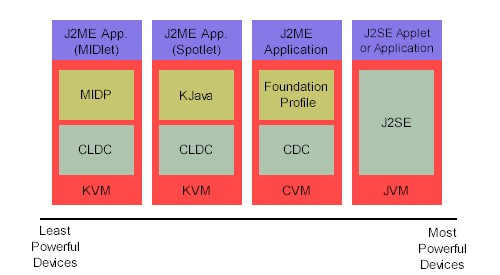
\includegraphics[width=.8\linewidth]{figures/j2me-architecture}
\end{center}
\caption{J2ME Architecture (from: `J2ME: Step by step' by IBM developerWorks).}%
\label{fig:j2mearchitecture}
\end{figure}

The modular design of the J2ME architecture enables an application to be scaled based on
constraints of a small computing device. J2ME architecture does not replace the operating
system of a small computing device. Instead, J2ME architecture consists of layers located
above the native operating system, collectively referred to as the Connected Limited
Device Configuration (CLDC). The CLDC, installed on top of the operating
system, forms the run-time environment for small computing devices.

\begin{figure}[t]%
\begin{center}
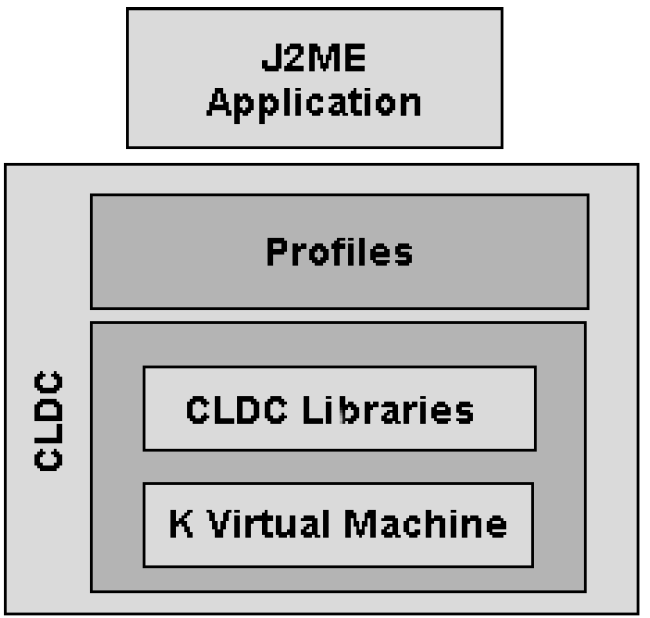
\includegraphics[height=6cm]{figures/j2me-architecture-2-b}
\end{center}
\caption{J2ME Architecture cd (from: `Wireless Programming with J2ME: Cracking the Code' by Dreamtech Software India, Inc., Team).}%
\label{fig:j2mearchitecture2}
\end{figure}

A \emph{MIDlet} is a J2ME application designed to operate on an MIDP small computing
device. A MIDlet is defined with at least a single class that is derived from the 
\texttt{javax\-.microedition\-.midlet\-.MIDlet} class.

\subsection{Event Handling}

A MIDlet is an event-based application. All routines executed in the MIDlet are invoked
in response to an event reported to the MIDlet by the application manager. The initial
event that occurs is when the MIDlet is started and the application manager invokes the
\texttt{startApp()} method.

The \texttt{startApp()} method in a typical MIDlet contains a statement that displays a screen
of data and prompts the user to enter a selection from among one or more options. The
nature and number of options is MIDlet and screen dependent.

A \texttt{Command} object is used to present a user with a selection of options to choose
from when a screen is displayed. Each screen must have a \texttt{CommandListener}. A \texttt{CommandListener}
monitors user events with a screen and causes the appropriate code to execute based on the current event.

\subsection{User Interfaces}

The design of a user interface for a MIDlet depends on the restrictions of a small
computing device. Some small computing devices contain resources that provide
a rich user interface, while other more resource-constrained devices offer a modest
user interface. A rich user interface contains the following elements, and a device
with a minimal user interface has some subset of these elements as determined by
the profile used for the device.

A \texttt{Form} is the most commonly invoked user interface element found in a MIDlet
and is used to contain other user interface elements. Text is placed on a form as a
\texttt{StringItem}, a \texttt{List}, a \texttt{ChoiceGroup}, and a \texttt{Ticker}.

A \texttt{StringItem} contains text that appears on a form that cannot be changed by the
user. A \texttt{List} is an itemized options list from which the user can choose an option. A
\texttt{ChoiceGroup} is a related itemized options list. And a \texttt{Ticker} is text that is scrollable.

A user enters information into a form by using the \texttt{Choice} element, \texttt{TextBox},
\texttt{TextField}, or \texttt{DateField} elements. The \texttt{Choice} element returns an option that the user
selected. \texttt{TextBox} and \texttt{TextField} elements collect textual information from a user and
enable the user to edit information that appears in these user interface elements. The
\texttt{DateField} is similar to a \texttt{TextBox} and \texttt{TextField} except its contents are a date and time.

An \texttt{Alert} is a special case of a \texttt{Form} that is used to alert the user that an error has occurred.
An \texttt{Alert} is usually limited to a \texttt{StringItem} user interface element that defines the
nature of the error to the user.

To use the display and the low-level user interface API directly, the developer should use the \texttt{Graphics}
and \texttt{Canvas} classes.
The \texttt{Canvas} class provides the display surface, its dimensions, and callbacks used to handle key and pointer events
and to paint the display when requested. The methods of this class must be overridden by the developer to respond
to events and to paint the screen when requested. The \texttt{Graphics} class provides methods to paint lines, rectangles,
arcs, text, and images to a \texttt{Canvas} or an \texttt{Image}. To gain access to even more low-level events a programmer
can use \texttt{GameCanvas} class that is direct subclass of Canvas.


\chapter{RobotME Framework Design}

We divided the problem into fairly independent goals. The first goal was to design a mechanism
that would allow us to intercept and record the events resulting from user's interaction with the
program (running on an emulator or a real device). This is called the \emph{recording phase}. The 
second goal was to programmatically simulate the previously recorded events (user actions) -- this is
called the \emph{replay phase}. Finally, we compare the initial recording with stimuli 
resulting from the replayed events; certain \emph{assertions} are checked to ensure the program followed
an identical sequence of state transitions (this implies a correct outcome of the entire test). Note
that states can be fairly low-level, such as action selection, but also high-level, perhaps even
explicitly hardcoded in the program under test by the developer. We took extra care to  
facilitate future maintenance of the recorded scripts. Unlike with desktop applications, 
where an event is typically described by a mouse position or some obscure component identifier, 
our events are described with names meaningful to the programmer (an action's label 
for example). Our goal is to make the recorded script comprehensible and comparable to a 
typical (unstructured) use-case scenario used in requirements engineering.


\section{Problems}
% subclassing, finalized classes/ methods, container environment.

The main problem is to capture and generate events of various GUI elements in a consistent, 
reliable manner, regardless of the techniques used by the program developer. We can distinguish
several different scenarios (each explained in detail further on):
\begin{itemize}
    \item \emph{subclassing} used to modify or extend the default behaviour of \texttt{Form}, \texttt{Canvas}, 
    \texttt{MIDlet} and other J2ME elements,
    
    \item \emph{direct use of an object} as in the case of the \texttt{Command} class,
    
    \item \emph{listeners} receiving callback events from \texttt{Form} and other 
    subclasses of \texttt{Displayable}.
\end{itemize}

Additional issues arise from the fact that the above scenarios may appear in different combinations
in the tested program's bytecode -- a bytecode instrumentation solution should detect and properly 
`wrap' such code to capture or generate events.  

Let us provide some more examples of real code and the way it is translated to Java bytecode.

\subsection{A \texttt{Command} object being added to a \texttt{Form}}\label{sect:fiugvuieg}

We must intercept every attempt to add a \texttt{Command} object to an existing screen, namely
the invocation of the \texttt{addCommand} method on \texttt{Displayable}). 
A programmer may add a command in many ways, for example by adding class-level 
static fields:

\begin{javablock}
public class ClassUnderTest {
    private static final Command MY_COMMAND = new Command("Cmd label", Command.OK, 1);

    public ClassUnderTest() {
        Form f = new Form("Title");
        f.addCommand(MY_COMMAND);
    }
}
\end{javablock}

\noindent%
At the bytecode level the above snippet looks as shown below:

\begin{javablock}
ALOAD 1
GETSTATIC ClassUnderTest.MY_COMMAND : Ljavax/microedition/lcdui/Command;
INVOKEVIRTUAL javax/microedition/lcdui/Displayable.addCommand(Ljavax/microedition/lcdui/Command;)V
\end{javablock}

\noindent%
This means: load first local variable onto the stack (\texttt{Form f}), load static class field onto the stack, 
invoke \texttt{addCommand} method of the \texttt{Displayable} instance with the arguments from the stack.
A different attempt to do the same thing is using object-level fields:

\begin{javablock}
public class ClassUnderTest {
    private final Command MY_COMMAND = new Command("Cmd label", Command.OK, 1);

    public ClassUnderTest() {
        Form f = new Form("Title");
        f.addCommand(MY_COMMAND);
    }
}
\end{javablock}

\noindent%
At the bytecode level this translates to:

\begin{javablock}
ALOAD 1
ALOAD 0
GETFIELD ClassUnderTest.MY_COMMAND : Ljavax/microedition/lcdui/Command;
INVOKEVIRTUAL javax/microedition/lcdui/Displayable.addCommand(Ljavax/microedition/lcdui/Command;)V
\end{javablock}

\noindent%
Which means: load first local variable onto the stack (\texttt{Form f}), load `this' variable (self reference) onto the stack,
load object-level field onto the stack (and in the same step remove `this' variable from the stack),
invoke the \texttt{addCommand} method of the \texttt{Displayable} instance with the arguments from the stack.

The second example is only slightly different from the first one. But it is possible to do the same thing in
completely different manner, using factory methods:

\begin{javablock}
public class ClassUnderTest {
    private static final Command getMyCommand() {
        return new Command("Cmd label", Command.OK, 1);
    }

    public ClassUnderTest() {
        Form f = new Form("Title");
        f.addCommand(getMyCommand());
    }
}
\end{javablock}

\noindent%
results in bytecode:

\begin{javablock}
ALOAD 1
INVOKESTATIC ClassUnderTest.getMyCommand()Ljavax/microedition/lcdui/Command;
INVOKEVIRTUAL javax/microedition/lcdui/Displayable.addCommand(Ljavax/microedition/lcdui/Command;)V
\end{javablock}

\noindent%
Yet another alternative is providing \texttt{Command} objects while adding it 
to the \texttt{Form}:

\begin{javablock}
public class ClassUnderTest {
    public ClassUnderTest() {
        Form f = new Form("Title");
        f.addCommand(new Command("Cmd label", Command.OK, 1));
    }
}
\end{javablock}

\noindent%
results in bytecode:

\begin{javablock}
ALOAD 1
NEW javax/microedition/lcdui/Command
DUP
LDC "Cmd label"
ICONST_4
ICONST_1
INVOKESPECIAL javax/microedition/lcdui/Command.<init>(Ljava/lang/String;II)V
INVOKEVIRTUAL javax/microedition/lcdui/Displayable.addCommand(Ljavax/microedition/lcdui/Command;)V
\end{javablock}

A more complex snippet could subclass the \texttt{Command} class (it has no real meaning here, but is
technically correct):

\begin{javablock}
public class ClassUnderTest {
    public ClassUnderTest() {
        Form f = new Form("Title");
        f.addCommand(new Command("Cmd label", Command.OK, 1) {
            public String getLabel() {
                return "Other Cmd label";
            }
        });
    }
}
\end{javablock}

\noindent%
compiles into:

\begin{javablock}
ALOAD 1
NEW ClassUnderTest$1
DUP
ALOAD 0
LDC "Cmd label"
ICONST_4
ICONST_1
INVOKESPECIAL ClassUnderTest$1.<init>(LClassUnderTest;Ljava/lang/String;II)V
INVOKEVIRTUAL javax/microedition/lcdui/Displayable.addCommand(Ljavax/microedition/lcdui/Command;)V
\end{javablock}


\subsection{Subclassing the \texttt{Form} class}

There are also cases that cannot be resolved by simply investigating compiled byte code once because of the complex
interdependencies between the standard API code and code created by the programmer. The only solution then is
having two-phase analysis of the compiled code: the first one creates a map of the interdependencies, and the second
looks for the appropriate injection points. For example, compare creating a \texttt{Form} screen by simply using 
its default constructor:

\begin{javablock}
Form f = new Form("Title");
\end{javablock}

\noindent%
to creating an instance of a derived class: 

\begin{javablock}
public class MyOwnForm extends Form {	
    public MyOwnForm(String s) {
        super(s);
    }
}

MyOwnForm f = new MyOwnForm("Title");
\end{javablock}

\noindent%
Creating the first object at the bytecode level looks like this:

\begin{javablock}
NEW javax/microedition/lcdui/Form
DUP
LDC "Title"
INVOKESPECIAL javax/microedition/lcdui/Form.<init>(Ljava/lang/String;)V
ASTORE 1
\end{javablock}

\noindent%
and creating the second object: 

\begin{javablock}
NEW MyOwnForm
DUP
LDC "Title"
INVOKESPECIAL MyOwnForm.<init>(Ljava/lang/String;)V
ASTORE 1
\end{javablock}

Note the second example has no direct relation with the standard J2ME API, therefore
it is impossible to tell only from this snippet of code what type of object
\texttt{MyOwnForm} really is. In the Java runtime we may use \texttt{instanceof} operation
to verify if \texttt{MyOwnForm} is a subclass of \texttt{Form} but it is impossible to do so while
statically investigating Java bytecode. Hence the need for two passes over bytecode -- one to 
determine inheritance hierarchy, the other for detecting potential event injection points.


\subsection{Injection points related to listeners}

Intercepting the addition and removal of listeners is required because we will need to
forward real GUI events to them after recording and artificially generated 
events at replay. The mechanism of intercepting the calls to \texttt{addCommandListener}
method is very similar to the one described previously in Section~\ref{sect:fiugvuieg},
so we omit its details here. An example of a code fragment adding a `self' object as 
a listener of a \texttt{Form} is given below:

\begin{javablock}
public class MyClass implements CommandListener {
    public MyClass(Form f) {
        f.addCommandListener(this);
    }
...
\end{javablock}


\subsection{Storage for recorded events}

An additional problem to solve in the recording phase was related to storage
of the recorded events. Saving all events directly on the device was inconvenient
because we could collide with the application's data or exceed the device's limited
capacity (memory or persistent storage). Eventually we decided to transmit all
events directly over the wire during the simulation and have an option to save
them locally in case network protocol is unavailable on the device.



\section{High-level Architecture}

When talking about high-level architecture we must distinguish several parts of the framework:

\begin{description}
    \item[Framework core] A group of classes used both during event capturing and
replaying. Contains most of the code that performs event capturing and forwarding 
events to the Log Server module.

    \item[Enhancer] A separate tool that gets as its input Java archive (JAR) file
with the compiled Java mobile applications and returns an `enhanced' version of the bytecode
with injected instructions related to the RobotME Testing Framework. 
It works in two modes: one dedicated to recording/ capturing phase that creates
enhanced JAR with injected code that is able to intercept user events;
second dedicated to replaying phase that creates enhanced JAR with injected code that
is able to simulate previously captured events.

    \item[Log Server] A tool that is deployed on some PC machine and is 
constantly listening for incoming messages from the mobile phone under test. It stores
received messages (events) from the mobile phone in the byte protocol format.

    \item[XML Processor] A tool for decoding the binary protocol
    with stored events and convert it into human-friendly XML form and vice versa.

    \item[Application under test] Not really part of the RobotME Testing Framework but an
    important element of the testing scenario; forms an input to the RobotME Testing Framework.
\end{description}

\begin{figure}[t]%
\begin{center}
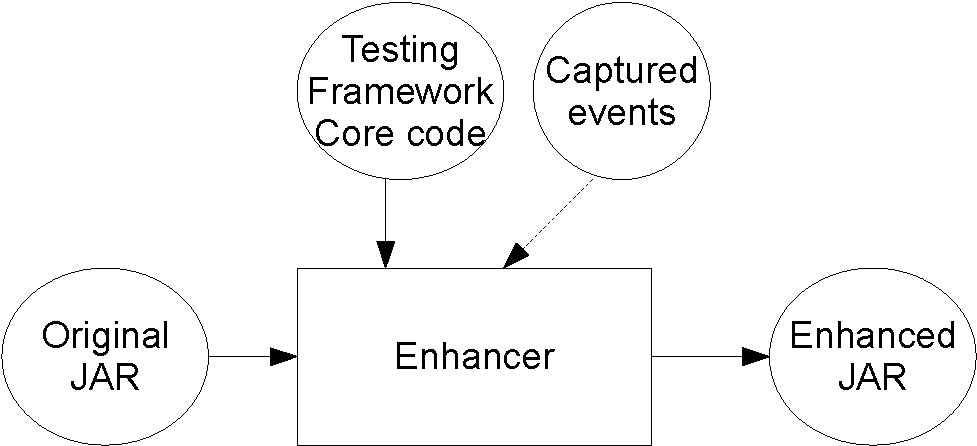
\includegraphics[width=.5\linewidth]{figures/diagram1}
\end{center}
\caption{Enhancement process.}%
\label{fig:diagram1}
\end{figure}

\begin{figure}[t]%
\begin{center}
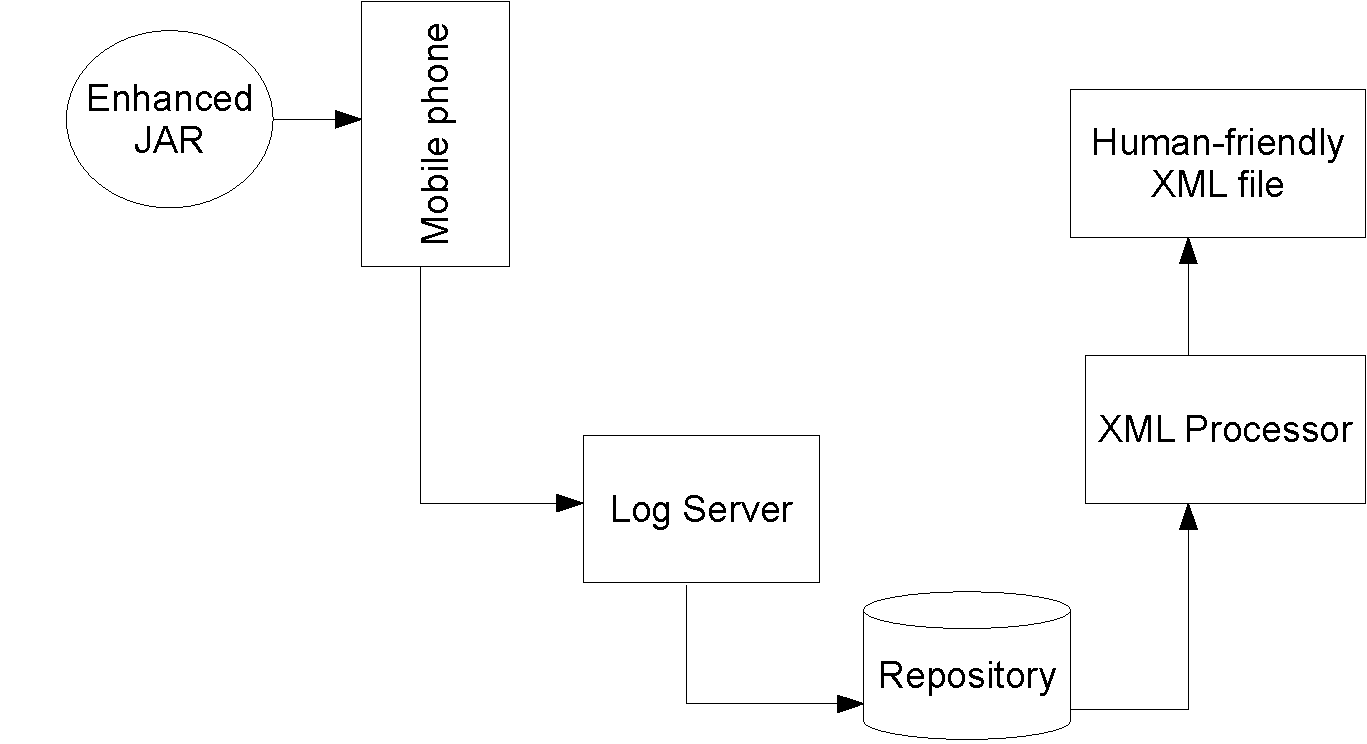
\includegraphics[width=.6\linewidth]{figures/diagram2}
\end{center}
\caption{Typical capturing/ replaying process.}%
\label{fig:diagram2}
\end{figure}

Going into further details of RobotME core architecture  (but still not going into
low-level implementation detail) several most important classes must be described and
interrelations between them. All of the important classes are depicted in 
Figure~\ref{fig:uml-diagram-1}.

\begin{figure}[p]%
\begin{center}
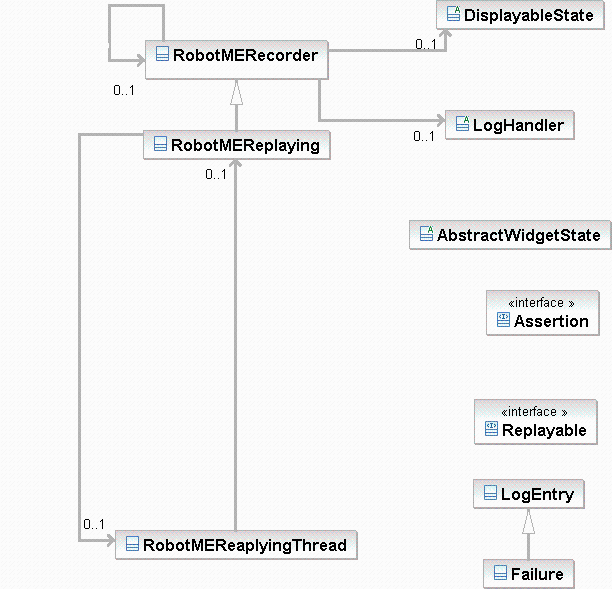
\includegraphics[width=\linewidth]{figures/uml-diagram-1}
\end{center}
\caption{Most important classes from RobotME core.}%
\label{fig:uml-diagram-1}
\end{figure}

\begin{description}
\item[RobotMERecorder] It is the central point of all of the framework activities and the only class
that is directly invoked from the injected code. It preserves all important information
about  the running Midlet like: connections between displaying screens and commands on them
and what screen is currently displayed.

\item[RobotMEReplaying] This class derives from the \texttt{RobotMERecorder} class because from the
capture-replay framework point of view replaying process is an extended version of recording process.
It is because during replaying process to be able to watch what is going on in the application
we must observe the application, therefor record each occurred events. Note that \texttt{RobotMEReplaying}
is used only during replaying process, but \texttt{RobotMERecorder} is used both during capturing
and replaying process. The important parts in which this class extend \texttt{RobotMERecorder} class
is mostly by adding ability of starting and stopping replaying process.

\item[RobotMEReaplyingThread] it is usual Java thread (derives from standard \texttt{Thread} class).
The responsibility of this class is to constantly read remaining events from the repository
(usually repository is plain file located in the same JAR as Midlet application) and simulate read events in
appropriate time intervals.

\item[DisplayableState] it is common knowledge that all action usually has some reaction (visible or not).
The same is with mobile application: all user or system-level actions (events) usually leads to some
reaction (both visible on the screen but not always). \texttt{DisplayableState} abstract class is the
way of storing all those reactions that are visible on the screen. There are many implementations
of this class: \texttt{AlertState}, \texttt{CanvasState}, \texttt{FormState}, 
\texttt{ListState} and \texttt{TextBoxState}. All screen
types existing in J2ME specification has its own \texttt{DisplayableState} implementation that
knows how to obtain and preserve state of such a screen.

\item[AbstractWidgetState] one of the screen types could have very complex internal state -- it is the
\texttt{Form} screen.
This kind of screen has its own implementation of \texttt{DisplayableState} -- a \texttt{FormState} class.
\texttt{FormState} implementation preserves only general information about \texttt{Form},
like its title and ticker text
(ticker is kind of scroll bar that is constantly scrolling some text on top or on the 
bottom of mobile phone screen). Forms as defined in the J2ME specification could have
so-called \texttt{Items} in it. The examples of predefined items are: simple labels, text fields, data fields,
choice groups (radio buttons or check-boxes), gauges, images and more, even custom items
(prepared entirely by the programmer, in current prototype implementation our testing
framework does not support this kind custom of Items). Each of this items has its own internal state, and
taken together form state of their parent Form. AbstractWidgetState abstract class
is the parent class for all of the implementations that store information
about internal states of the items. Some of the implementations are:
\texttt{ChoiceGroupWidgetState}, \texttt{DateFieldWidgetState}, \texttt{ImageItemWidgetState},
\texttt{TextFieldWidgetState} and
others. Each of implementation of \texttt{AbstractWidgetState} knows how to retrieve state
of its Item and how to preserve it (serialize to the event code).

\item[LogHandler] is the handler responsible for logs, for forwarding serialized events to appropriate
receiver. Examples of such receivers could be: remote PC with socket, bluetooth, infra-red
or serial connection, or even local (on the phone) receiver that stores events in the local
store (so called Record Store).

\item[LogEvent] is the base class for all kind of events possible to intercept during
program execution. Detailed list of every event types is presented in the next section.

\item[Replayable] is a base interface for implementation of class that are able to
simulate (replay) previously recorded events.

\item[Assertion] after each of simulated action state of the whole application is verified
(display screen, internal memory etc). This kind of verification is called assertion,
and if the verification process does not succeed Failure event is stored as the 
occurred event (it is kind of internal special purposes event).

\end{description}


\section{Recorded Event Types}

RobotME Testing Framework was created with the possibility of easily extending events set in mind.
In the current prototype implementation we were concentrated on implementing interception of most
occurred events, which are:
\begin{itemize}
\item  intercepting of modification of every kind of screens, also with complex 
\texttt{Canvas} and \texttt{Forms} (excluding custom items inside forms,
 it is possible to support such kind of items, but needs to introduce direct dependency between
 application under test and RobotME Testing Framework,
 it is subject to future extends),
\item  intercepting invocation of Commands actions,
\item  intercepting of low-level key events,
\item  intercepting of low-level pointer events.
\end{itemize}

This set of interceptors allows to test most of the currently existing mobile applications.

The other kind of interceptors that are planned to implement in the future:
\begin{itemize}
\item  intercepting modifications of the local record store,
\item  intercepting invocations of all phone calls,
\item  intercepting incoming and outgoing SMS, MMS i CBS messages,
\item  intercepting incoming and outgoing HTTP, socket, bluetooth and other kind of connections,
\item  intercepting sound events,
\item  intercepting every access to \texttt{System.out} and \texttt{System.err} streams.
\end{itemize}

Most of mobile phone hardware vendors have their own API to fulfill special needs like: LED lighting,
access to vibra or mobile phone contact book. We are not considering implementation of such
proprietary events, but left our RobotME Testing Framework open and it will be possible to
implement such events by the interested in them parties as a future extends.


\chapter{RobotME: Implementation}

\section{System Components}

As was outlined previously in the High-level Architecture section the main system components are:
Framework core itself, Enhancer, Log Server, XML Processor. There are no
separate components such as Recorder or Replayer (or more accurately: they are part of the
Framework core).

\subsection{Enhancer}
As was said in previous chapter, this component is a separate tool which gets an input Java archive (JAR) file
with the compiled Java mobile applications and returns `enhanced' the same Java archive
with the code related to the RobotME Testing Framework (specialized code is `injected' into original
JAR file). The Enhancer works in two modes: former represents recording/ capturing phase that creates
enhanced JAR with injected code that is able to intercept the user events;
and the latter represents replaying phase that creates enhanced JAR with injected code that
is able to simulate the previously captured events.

From the implementation point of view the Enhancer is a separate Java J2SE program, which is implemented as an ANT
task (so it can work as a stand-alone tool from the console and as part of the build process). The basic responsibility
of this tool is to investigate the compiled Java code of the input JAR file. The tool intercepts appropriate
parts of the code (in Aspect Oriented Programming these are called join points), modify them in expected way
and put back to the output JAR file.

The Java bytecode is a kind of assembler language with low-level opcodes. It is very difficult to investigate
such a code and find an appropriate places for interception. To do this the programmer
should feel comfortable with the great amount of different mnemonics of Java (There are between
200 and 256 mnemonics, depending on how the JVM has enhanced the standard
set with optimizing extensions). 
To simplify the work with bytecode there are various
aspect-oriented frameworks like AspectJ, AspectWerkz 
or even Spring Framework build-in AOP facility. Unfortunately these frameworks do not offer enough
expressive power to describe the injection points we mentioned earlier.
There is a finite set of transformations that AOP (aspect-oriented programming)
techniques can do (for example Spring Framework AOP mechanism creates only
proxies for classes it transforms; AspectJ can include various Java code inside Java methods,
but it also includes code strictly dependent to its own API which is not acceptable
-- mobile applications must be as small as possible). Due to all of these problems
we decided not to use the AOP frameworks at all. We concentrated on the Java bytecode modification
frameworks that offer not only more low-level access to the modifying bytecode but also offer
some help with transformations techniques. To our knowledge there are two most often
used open-source frameworks that fulfill such requirements: ASM and Apache
BCEL. Both of these frameworks were thoroughly
tested and verified. We have chosen ASM as a foundation for our Enhancer.
The choice was made because of:
\begin{itemize}
\item the company which supports ASM, France Telecom R\&D Center, guarantees good quality of the product;
\item ASM has substantially smaller memory and computation overhead compared to BCEL;
\item ASM is easier to use and covers both tree-like investigation of the Java bytecode as well as
  event-like (similarly to XML code parsing where these terms are called: DOM and SAX techniques respectively).
\end{itemize}

Having chosen bytecode modification framework we created base Enhancer architecture around the ASM
framework and its processing scheme which is based on visitor design pattern (event-like). The internal 
Enhancer's architecture is depicted on the class diagram on Figure~\ref{fig:uml-diagram-enhancer}.

\begin{figure}[t]%
\begin{center}
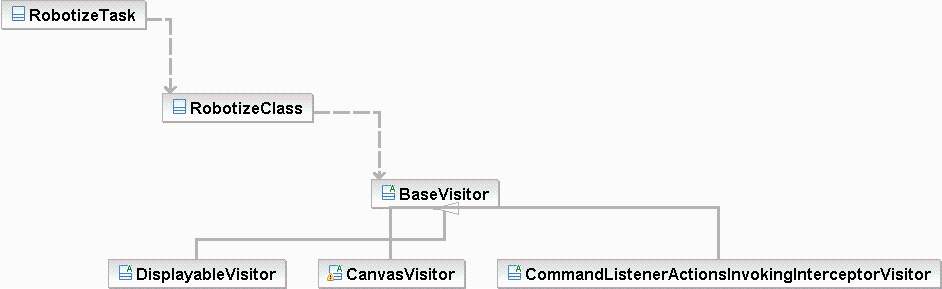
\includegraphics[width=\linewidth]{figures/uml-diagram-enhancer}
\end{center}
\caption{The implementation of Enhancer.}%
\label{fig:uml-diagram-enhancer}
\end{figure}

The presented classes are responsible for:

\begin{description}
    \item[RobotizeTask] it is the ANT task and entry point of the Enhancer tool. RobitizeTask has reference to the 
\code{RobotizeClass}.

    \item[RobotizeClass] is the main class responsible for delegating enhancing task to the appropriate utility components
 including: decompressing JAR file, iterating over Java class files, writing transformated bytecode to the
 Java class file, compressing back previously transformated code to the output JAR file.

    \item[BaseVisitor] each of transformation type is implemented in its own separate Java class and BaseVisitor
forms a base implementation for all of transformations and offer most frequently used methods like 
obtaining Java bytecode and managing lifecycle of the transformation process. It has many specific
implementations some of them are depicted on the diagram as classes that derives from it.
\end{description}

\subsection{Recorder}

The Recorder starts working when the mobile application (Midlet) begins execution inside
the KVM. The code injected into the original application calls internal classes 
of the RobotME core forwarding the required events. 

The main application's midlet is wrapped in the \texttt{RobotMERecorder} class. 
It is a singleton class and only one instance
of this class exists per one running mobile application. The framework is able to differentiate
between low-level events (key presses, pointer movements) and high-level events (commands invoked 
by the user). These events are passed to cooperating objects like: implementations of the \texttt{DisplayableState}
class and \texttt{LogHandler} and further to the Log Server component. 

There are cases when an event that occurred in the mobile application does not leave any changes
in the internal state of the mobile application. It is also \texttt{RobotMERecorder}'s responsibility
to detect such situations and react accordingly (log an intercepted event but with the
information that it is not candidate for the assertion verification because it leads
to no visible internal state changes).

\subsection{Replayer}

Replayer is an extended version of the recorder component (reason to such a case was mentioned in
the high-level architecture chapter). From the framework's internals point of view the Replayer is
really two cooperating things: one, a Java thread that constantly reads events from
repository (in current prototype implementation only files bundled into JAR file
are supported as repository). Based on a read event (\texttt{LogEntry}), this thread creates corresponding
\texttt{Replayable} object that knows how to replay a given \texttt{LogEntry}. The second
thing is \texttt{RobotMEReplaying} class. Reponsibility of this class is similar to
\texttt{RobotMERecorder} -- to intercept every event interesting from the RobotME Testing Framework
point of view and perform verification of the internal mobile application state.
If state of the mobile application violates those that was stored in the
application usage scenario assertion is triggered (assertions are further described
in Section~\ref{sect:assertionsandfailurenot}). If state of the mobile
application is as expected simulator runs without stopping itself.

\subsection{Log Server}

Log Server is another separate Java J2SE tool (similarly to the enhancer component). It works on desktop
machine and its responsibility is to constantly listening for the incoming events from the
mobile programs under test and then store each received event (not interpreting them). Log Server is 
internally dependent on the Framework Core component and uses some of its classes, mainly
as events encapsulations.

\begin{figure}[t]%
\begin{center}
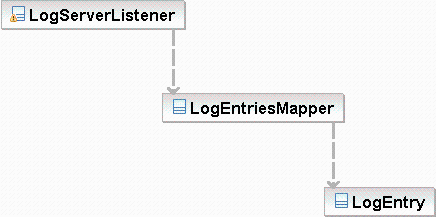
\includegraphics[width=.7\linewidth]{figures/uml-diagram-logserver}
\end{center}
\caption{Log Server implementation.}%
\label{fig:uml-diagram-logserver}
\end{figure}

Log Server architecture consists of one main class:
\texttt{LogServerListener}, that internally creates separate thread for each incoming
connections from the mobile application under test, therefor is able to receive
separate events from separate mobile applications, each connection not
interfere with any other (one connection per remote device).

\texttt{LogServerListener} is build in the way that it can be abstracted from the nature of
the underlying connection. It does not matter if the connection is performed as
a bluetooth or infra-red transfer, GPRS internet transfer or even simply
serial port connection (but what is usually important for the users is a price,
some of above connections are free of charge while the others might not be).
LogServerListener treat each connection type in the same manner -- as a form
of events transfer channel.

\texttt{LogEntriesMapper} -- is a class that knows how to create \texttt{LogEntry} class instance
from the received by \texttt{LogServerListener} event. Each \texttt{LogEntry} and also each event
are distinguishable by its unique ID number. To allow future implementations of
other special events (for example Nokia phones specific events) each ID
has its prefix and every internal events implemented as a part of the core RobotME Testing
Framework has its own reserved prefix. There is also a reserved prefix for custom,
third parties event IDs.

\subsection{XML Processor}

XML Processor is yet another separate Java J2SE tool. It is responsible for converting
stream of events (stored as a compact binary protocol) to the human-friendly
XML form of events. Its other task is to convert events back from human-friendly
XML form into compact binary protocol ready to replay on the mobile application.

Classes that take part in this processes are depicted on the following diagram.

\begin{figure}[t]%
\begin{center}
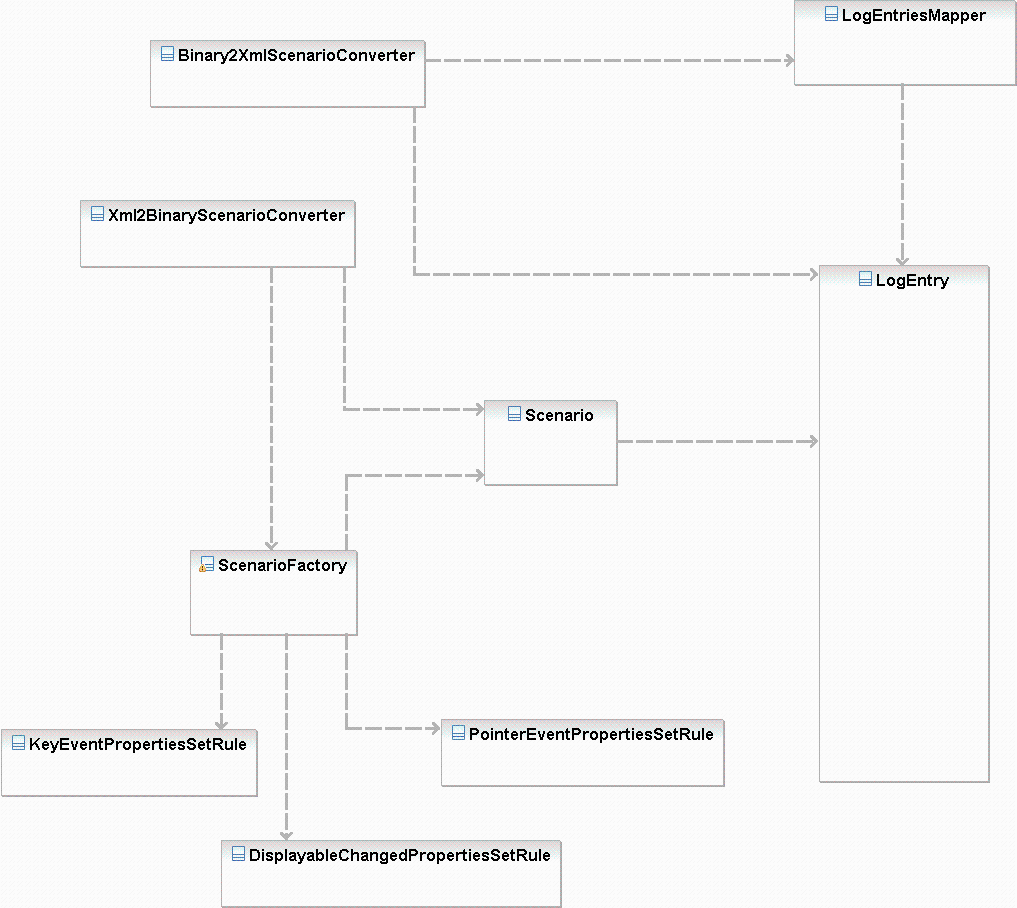
\includegraphics[width=\linewidth]{figures/uml-diagram-xmlprocessor}
\end{center}
\caption{XML Processor implementation.}%
\label{fig:uml-diagram-xmlprocessor}
\end{figure}

\texttt{Scenario} is a class that stores list of \texttt{LogEntries} that as a whole
form a usage scenario of an associated mobile application. In its internal
nature Scenario is very simple class, but fulfill important requirements.
Having scenario object with \texttt{LogEntries} in appropriate order in it you
know how mobile application is intended to use, therefor you can simulate
it.

\texttt{ScenarioFactory} is a factory method design pattern class that as an input takes two things:
XML file with the payload of occurred events in the mobile application
and a set of rules that describe how to transform XML constructions
into list of \texttt{LogEntry} objects that will form \texttt{Scenario} object. Currently association
of ScenarioFactory and a set of rules is hardcoded in the \texttt{ScenarioFactory} class, but it is
done in very straightforward manner and it will be easy to move this association
description to some configuration file. Thanks to it it will be simple
for the third party companies that will want to add they own events in the RobotME Testing Framework
in the future to do so just by modifying configuration file.

\texttt{Xml2BinaryScenarioConverter} and \texttt{Binary2XmlScenarioConverter} are two complementary 
converters that perform conversions from XML scenario format into
compact binary format and vice versa. The first of them realizes its task
by delegating internals of the conversion to \texttt{ScenarioFactory} class
while the second uses \texttt{LogEntriesMapper} capabilities of creating
\texttt{LogEntry} objects out of the binary protocol and \texttt{LogEntry} capability
to convert itself into XML format event.


\section{Examples of modifications introduced to the bytecode}

In this section we demonstrate actual bytecode transformations introduced to the
mobile application by the RobotME prototype.

\subsection{Intercepting subclasses}

Intercepting subclassing is particularly important in case of  mobile applications that 
make use of custom subclasses of the \texttt{Canvas} class. An example code that
uses the \texttt{Canvas} could look like this:

\begin{javablock}
class MyCanvas extends Canvas {

	protected void paint(Graphics g) {
        // painting goes here
	}

	protected void keyPressed(int keyCode) {
		System.out.println("In keyPress");
	}

    // ... handling of other events
}
\end{javablock}

\noindent%
After bytecode transformation and reverse-engineering to the source code, the
above snippet looks like this:

\begin{javablock}
class MyCanvas extends Canvas {

	protected void paint(Graphics g) {
        // painting goes here
	}

	protected void keyPressed(int keyCode) {
		RobotMERecorder.getRecorderInstance()
            .keyEventOnCanvas(KeyEventOnCanvasLogEntry.KEY_PRESSED_TYPE, keyCode);
		$robotized$keyPressed(keyCode);
	}

	private final void $robotized$keyPressed(int keyCode) {
		System.out.println("In keyPress");
	}
// handling possibly other events
}
\end{javablock}

The original code for handling key press event was moved from method \texttt{keyPressed} to
method \texttt{\$robotized\$keyPressed} (these are private and final
methods to prevent overriding in further subclasses). In the \texttt{keyPressed} method 
we add an invocation of the oryginal key press handling code and also delegate to our framework code.

Below is the same transformation shown at the bytecode level. First the original class:

\begin{javablock}
public class org/example/midlet/canvas/MyCanvas extends javax/microedition/lcdui/Canvas  {

  public <init>()V
    ALOAD 0
    INVOKESPECIAL javax/microedition/lcdui/Canvas.<init>()V
    RETURN

  protected paint(Ljavax/microedition/lcdui/Graphics;)V
    RETURN

  protected keyPressed(I)V
    GETSTATIC java/lang/System.out : Ljava/io/PrintStream;
    LDC "In keyPress"
    INVOKEVIRTUAL java/io/PrintStream.println(Ljava/lang/String;)V
    RETURN
}
\end{javablock}

\noindent%
And after the transformation:

\begin{javablock}
public class org/example/midlet/canvas/MyCanvas extends javax/microedition/lcdui/Canvas  {

  public <init>()V
    ALOAD 0
    INVOKESPECIAL javax/microedition/lcdui/Canvas.<init>()V
    RETURN

  protected paint(Ljavax/microedition/lcdui/Graphics;)V
    RETURN

  protected keyPressed(I)V
    INVOKESTATIC org/robotme/core/recorder/RobotMERecorder
        .getRecorderInstance()Lorg/robotme/core/recorder/RobotMERecorder;
    ICONST_1
    ILOAD 1
    INVOKEVIRTUAL org/robotme/core/recorder/RobotMERecorder.keyEventOnCanvas(BI)V
    ALOAD 0
    ILOAD 1
    INVOKESPECIAL org/example/midlet/canvas/MyCanvas.$robotized$keyPressed(I)V
    RETURN

  private final $robotized$keyPressed(I)V
    GETSTATIC java/lang/System.out : Ljava/io/PrintStream;
    LDC "In keyPress"
    INVOKEVIRTUAL java/io/PrintStream.println(Ljava/lang/String;)V
    RETURN
}
\end{javablock}


\subsection{Intercepting \texttt{Command} events}

A snippet of Java code with a \texttt{Command} object being added to a \texttt{Form} could
look as shown below:

\begin{javablock}
Form form;
form.addCommand(CMD_OK);
\end{javablock}

\noindent%
After transformations it will look like this:

\begin{javablock}
Form form;
form.addCommand(CMD_OK);
RobotMERecorder.getRecorderInstance().commandAddedToDisplayable(CMD_OK, form);
\end{javablock}

We passed both \texttt{Displayable} and \texttt{Command} object to our core class. The same transformation
at the bytecode level is presented below.

\noindent%
Original code:

\begin{javablock}
ALOAD 1
GETSTATIC org/example/midlet/form/FormExampleMIDlet.CMD_OK : Ljavax/microedition/lcdui/Command;
INVOKEVIRTUAL javax/microedition/lcdui/Displayable.addCommand(Ljavax/microedition/lcdui/Command;)V
\end{javablock}

\noindent%
and after the transformation:

\begin{javablock}
ALOAD 1
GETSTATIC org/example/midlet/form/FormExampleMIDlet.CMD_OK : Ljavax/microedition/lcdui/Command;
INVOKEVIRTUAL javax/microedition/lcdui/Displayable.addCommand(Ljavax/microedition/lcdui/Command;)V
INVOKESTATIC org/robotme/core/recorder/RobotMERecorder
    .getRecorderInstance()Lorg/robotme/core/recorder/RobotMERecorder;
GETSTATIC org/example/midlet/form/FormExampleMIDlet.CMD_OK : Ljavax/microedition/lcdui/Command;
ALOAD 1
INVOKEVIRTUAL org/robotme/core/recorder/RobotMERecorder
    .commandAddedToDisplayable(Ljavax/microedition/lcdui/Command;Ljavax/microedition/lcdui/Displayable;)V
\end{javablock}


\subsection{Intercepting listeners}

Intercepting the code that associates listener objects with \texttt{Displayable} is in theory
very simillar to intercepting commands. 

\begin{javablock}
public class SampleClass implements CommandListener {
	public SampleClass() {
		TextBox textBox;
		textBox.setCommandListener(this);
	}

    // ...
}
\end{javablock}

\noindent%
After the transformation this code will be transformed into:

\begin{javablock}
public class SampleClass implements CommandListener {
	public SampleClass() {
		TextBox textBox;
		textBox.setCommandListener(this);
		RobotMEReplaying.getReplayingInstance().commandListenerSetOnDisplayable(this, textBox);
	}

    // ...
}
\end{javablock}

\noindent%
At the bytecode level the above is translates to:

\begin{javablock}
ALOAD 2
ALOAD 0
INVOKEVIRTUAL javax/microedition/lcdui/Displayable
   .setCommandListener(Ljavax/microedition/lcdui/CommandListener;)V
\end{javablock}

\noindent%
And after the transformation:

\begin{javablock}
ALOAD 2
ALOAD 0
INVOKEVIRTUAL javax/microedition/lcdui/Displayable
    .setCommandListener(Ljavax/microedition/lcdui/CommandListener;)V
INVOKESTATIC org/robotme/core/replaying/RobotMEReplaying
    .getReplayingInstance()Lorg/robotme/core/replaying/RobotMEReplaying;
ALOAD 0
ALOAD 2
INVOKEVIRTUAL org/robotme/core/replaying/RobotMEReplaying
    .commandListenerSetOnDisplayable(
        Ljavax/microedition/lcdui/CommandListener;
        Ljavax/microedition/lcdui/Displayable;)V
\end{javablock}


\section{Assertions and Failure Notification}\label{sect:assertionsandfailurenot}

Each time the \texttt{Replayer} component detects the difference between what was expected 
and what actually happened, a state assertion is triggered. \texttt{Assertion} is the base 
interface which must by implemented by each
class that knows how to verify the mobile application's state (in some part).

Because some of the verification tasks are common across all assertions
we decided to introduce an abstract class called \texttt{BaseAssertions}
that contains the common code. There are also several concrete implementations
of this class. For example one assertion verifies the content of \texttt{List} displayed on the screen.
There may exist other implementations that verify midlet record store contents, state of connections
to remote servers or even time of the local timer if it might be of importance).

\begin{figure}[t]%
\begin{center}
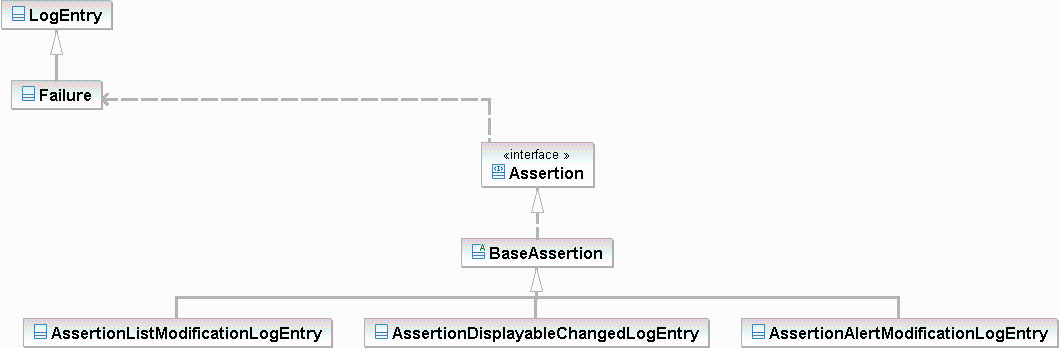
\includegraphics[width=\linewidth]{figures/uml-diagram-assertions}
\end{center}
\caption{Assertions implementation.}%
\label{fig:uml-diagram-assertions}
\end{figure}

Every time an assertion is violated a \texttt{Failure} object is created. This class is a subclass of
\texttt{LogEntry} and can be serialized to the binary protocol and transfered to the
Log Server component over a network connection. 

In the current prototype implementation of the RobotME framework there is only one action associated with
failures: terminate the whole mobile application and send every intercepted events to the
Log Server along with the Failure object itself. Then the real cause of the assertion
violations might be further investigated by the tester.

We are considering extending assertions so that there will be two types of them:
\begin{itemize}
    \item \emph{strong assertions} -- the same as in current implementation,
    \item \emph{weak assertion} -- violation of such assertion will not cause the whole mobile
  application to terminate, but only appropriate Failure object will be 
  transfered to the Log Server component. Sometimes this kind of assertions might
  be helpful with finding more errors in program execution than will be discovered
  only with strong assertions. Using this type of assertion we must be sure that after violation of
  weak assertion program will always be in consistent state, not causing
  further errors because of the weak assertion violation.
\end{itemize}


\chapter{Experiments and Evaluation}

\section{Lab Tests}

Parallel to building prototype RobotME Framework we were also building mobile application
that can be used to verify our framework capabilities. This application use each
kind of visual component with each possible features that the testing framework
supports.

Most of our tests were performed on emulators of real devices, usually using
generic emulator provided by Sun Microsystem called WTK (Wireless Toolkit) but also
SonyEricsson's and Nokia emulators. It was
because it is the fastest way of deploying mobile application and than executing it,
and during constant development there is simply no time for time consuming
deployment on real devices. After the prototype was created we performed several tests on 
real devices, including: SonyEricsson P900i (that supports CLDC 1.1 standard) and
SonyEricsson K610i (that on the other hand supports CLDC 1.0 standard). Our framework
supports all mobile devices that conforms to at least standards: MIDP 2.0 and
CLDC 1.0 so theoretically these two devices should be fully supported by RobotME
Framework.

Testing devices were connected to the Log Server through GPRS connection. For each of
visual component our framework supports dedicated scenarios were recorded. Then
we tried to replay previously recorded scenarios. When replaying scenario finishes
with success (no assertion was violated) then we modified scenario so that it should no longer
be correct and hoping that during next replaying process assertions will be violated
and tests will not pass. It was indeed in our case. All of tests passed when it
intended to, and all assertions was violated when we manually modified scenarios.

The example of one event that could be modified in the scenario so that whole scenario
will not pass could be as follows. It presents snapshot of states items on the form
that is currently shown on the device's screen.

Before modification:

\begin{xmlblock}
	<event level="INTERNAL" timestamp="1166970731531"
		replayable="false" assertion="true">
		<form-modification title="Form Title 1">
			<items>
				<choice-group label="Choice group label">
					<selectedFlags>
						<value>true</value>
						<value>false</value>
						<value>true</value>
					</selectedFlags>
					<strings>
						<value>Option 1</value>
						<value>Option 2</value>
						<value>Option 3</value>
					</strings>
				</choice-group>
				<date-field label="Date 1" date="1166970731529" />
				<gauge label="Gauge 1" value="6" />
				<image label="Img 1" altText="Alternative text 1" />
				<spacer />
				<string-item label="String item 1" text="Text 1" />
				<text-field label="Text field 1" string="String 1" />
			</items>
		</form-modification>
	</event>
\end{xmlblock}

After modification (form title was changed):

\begin{xmlblock}
	<event level="INTERNAL" timestamp="1166970731531"
		replayable="false" assertion="true">
		<form-modification title="Form Title 2">
			<items>
				<choice-group label="Choice group label">
					<selectedFlags>
						<value>true</value>
						<value>false</value>
						<value>true</value>
					</selectedFlags>
					<strings>
						<value>Option 1</value>
						<value>Option 2</value>
						<value>Option 3</value>
					</strings>
				</choice-group>
				<date-field label="Date 1" date="1166970731529" />
				<gauge label="Gauge 1" value="6" />
				<image label="Img 1" altText="Alternative text 1" />
				<spacer />
				<string-item label="String item 1" text="Text 1" />
				<text-field label="Text field 1" string="String 1" />
			</items>
		</form-modification>
	</event>
\end{xmlblock}

Please note that the same event XML definition could be used as an assertion
(if appropriate attributes are set to: replayable="false" assertion="true") but also
could be used to simulate user interaction with the mobile application
(if this attributes are set to: replayable="true" assertion="false").

\section{Real-life Use Case}

\begin{figure}[t]%
\begin{center}
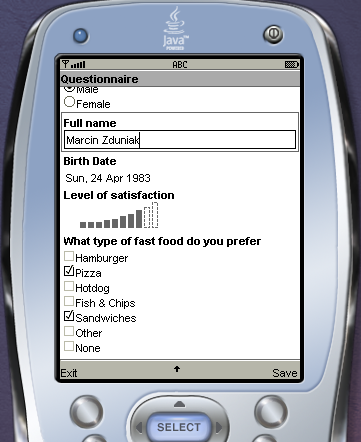
\includegraphics[width=.6\linewidth]{figures/screen-1b-emulator}
\end{center}
\caption{Emulator window with example mobile application under test.}%
\label{fig:screen-1b-emulator}
\end{figure}

\begin{figure}[t]%
\begin{center}
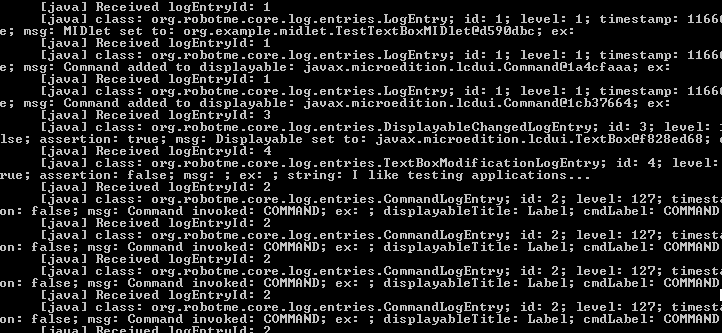
\includegraphics[width=\linewidth]{figures/screen-2-console}
\end{center}
\caption{Server console -- Log Server.}%
\label{fig:screen-2-console}
\end{figure}

As we were starting our work on this framework we were not sure if our idea is
even possible to realize and implement, there are no similar frameworks
for mobile platforms created before. We started from creating code that is
able to intercept events from the mobile phone as well as correctly
simulate them. Our prototype demonstrated it is possible.

The next thing that is still in front of us is verifying our framework against
real mobile application, that is not only a set of related screens created by
us to only demonstrate some Frameworks capabilities, but that that
have some useful logic behind this screens. Natural choice for candidate of such
application is NaviExpert, application created by group of researchers and
students from Poznan University of Technology intended to navigate simple
mobile phone users from one point to the other using back-end server and
GPS connected to the phone or embedded into mobile device. At this moment our prototype
solution is not ready to capture all important events in NaviExpert and
properly replay them. The points that must be addressed before being able to
test that application are:

\begin{itemize}
\item more kind of assertions need to be implemented, especially those related to 
  Record Store, sound events and various means of data transferring over the air like:
  bluetooth or GPRS connections.
\item tool that could visualize XML files with captured events so that editing
  it will be much easier and less error prone. Because in NaviExpert there
  are lot of events, even simple scenario is very long, difficult
  to understand and modify accordingly.
\end{itemize}

\section{Bytecode Size and Performance Aspects}

After enhancing process input JAR is substantially increased in size. The testing JAR size with sample application
is $34\,000$ bytes. Enhancing process increases JAR in two ways: one is an outcome of injecting code into existing classes
and the other is an outcome of adding RobotME Framework core classes to an existing application.
Testing JAR file after enhancement process that turns input mobile application into `capturing'
version has size: $120\,434$ ($71{,}7$\% increase), and `replaying' version: $121\,166$ ($71{,}9$\%).
Summarizing only the code that was injected (without RobotME Framework core classes) the numbers was as
follow:
\begin{itemize}
\item `capturing' version: $35\,853$ ($5{,}1$\%)
\item `replaying' version: $36\,585$ ($7{,}0$\%)
\end{itemize}

The differences (small but noticeable) leads from the fact that `replaying' version of the application
does exactly the same what `capturing' version of the application is doing plus some other extra
tasks.

The testing framework has different performance overhead depending if it is
in the capture or in replay mode. In the capture mode the overhead is mostly
bound to network traffic (sending events over the wire), which can be easily
neglected by using some engineering tricks (asynchronous queue of events waiting
to be sent). In the replay mode the overhead is connected to the background
thread reading and stimulating events. We found this overhead negligible as
well.

\section{Obfuscation}

% Does the injected code obfuscate? Is there anything interesting about it?

Both injected code and RobotME Framework API obfuscate to some extent. The testing application
input JAR after obfuscation takes $26\,210$ bytes, enhanced `capturing' version of the application
has $93\,237$ ($71{,}8$\%) bytes in size, and `replaying' version has: $93\,861$ ($72$\%).
Summarizing only the code that was injected (without RobotME Framework core classes) the numbers was as
follow:
\begin{itemize}
\item `capturing' version: $27\,473$ ($4{,}6$\%)
\item `replaying' version: $28\,097$ ($6{,}7$\%)
\end{itemize}


\chapter{Summary and Conclusions}

\section{Summary}

% Remind the reader what was planned. Sum up what's been achieved and what hasn't (and why)?

This thesis is a proof of concept demonstrating that fully-fledged capture-replay
testing framework is feasible in Java 2 Micro Edition environment. The
prototype implementation has been written for it and showed usable in practice. 
The framework may be used both in fully automated testing environments
exploiting mobile device simulators and in real environments with real
mobile devices.

Parts of this thesis have been published at the 10th International Conference on 
Business Information Systems, Poznan, Poland~\cite{zduniak-weiss-2007}.


\section{Future Directions}

Our biggest challenge at the moment is to provide some objective means to
assess the value gained from using the framework. What common sense states
as obvious is quite difficult to express with hard numbers. We considered a controlled
user experiment where participants would be given the same application
and a set of tasks to implement (refactorings and new features). Half of the
group would have access to the results of integration tests, the other half would
just work with the code. We hoped this could demonstrate certain gains (number
of early detected bugs, for example) that eventually translate into economic
value for a company. Unfortunately, this kind of experiment is quite difficult to
perform and its results are always disputable (i.e., due to ranging skills between
programmers), so we decided to temporarily postpone it. Other possible research
and technical directions are:
\begin{itemize}
    \item Design a flexible architecture adding support for events that are outside
the scope of the J2ME specification, but are commonly used in mobile development.
These events include, for example, vendor-specific APIs such as
vibration or backlight provided by Nokia.
    \item Implement alternative event serialization channels –- through serial cables or
Bluetooth connections.
    \item Consider evaluation schemes for the presented solution. A real feedback from
developers translates into a proof of utilitarian value of the concept -– does
the testing framework help? How much time/ work does it save? What is
the ratio of time spent on recording/ correcting test scripts compared to
running them manually? We should emphasize that these questions are just
as important as they are difficult to answer in a real production environment.
    \item Integrate the framework with popular integrated development environments.
This goal is very important because developers must be comfortable with the
tool to use it and must feel the benefits it provides. Instant hands-on testing
toolkit would certainly assimilate faster in the community than an obscure
tool (such as Sony’s).
    \item We also think about extending the concepts presented in this paper to other
Java-based platforms for building mobile applications, such as NTT DoCoMo
Java, BlackBerry RIM API or Qualcomm Brew. They may not be as popular
as J2ME, but the concepts we have presented should be applicable in their
case as well.
    \item Based upon the experience and feedback from the initial prototype, we asses there is a real demand
    and market need for such a testing tool. Writing a production-quality utility from
    scratch (that developers and testers could use with little knowledge of the internal mechanisms) 
    is a promising direction  for future work.
\end{itemize}


% All appendices and extra material, if you have any.
\cleardoublepage\appendix%
%\input{0a-appendix.tex}

% Bibliography (books, articles) starts here.
\bibliographystyle{alpha}{\raggedright\sloppy\small\bibliography{bibliography}}

% Web resources
\chapter*{List of Web Resources}\label{sect:web-resources}%
\phantomsection\addcontentsline{toc}{chapter}{Web Resources}

\newcommand{\tturl}{\begingroup \urlstyle{tt}\Url}

{\small
\begin{enumerate}[{[}A{]}]
    \item \label{unicode} The Unicode standard.\\
          \tturl{http://www.unicode.org}

    \item \label{j2meunit} J2MEUnit\\
          \tturl{http://j2meunit.sourceforge.net}

    \item \label{mobilejunit} Mobile JUnit, Sony Ericsson\\
          \tturl{http://developer.sonyericsson.com/getDocument.do?docId=87520}

    \item \label{rational} TestRT (Rational Test RealTime), IBM\\
          \tturl{http://www.ibm.com/software/awdtools/test/realtime/}

    \item \label{bbfledge} Fledge (Java Development Environment and BlackBerry Fledge simulator), Research in Motion\\
          \tturl{http://na.blackberry.com/eng/developers/downloads/jde.jsp}

    \item \label{gatling} Gatling, Motorola\\
          \tturl{https://opensource.motorola.com/sf/sfmain/do/viewProject/projects.gatling}

    \item \label{cldcunit} CLDCUnit, Pyx4me\\
          \tturl{http://pyx4me.com/snapshot/pyx4me/pyx4me-cldcunit/}

\end{enumerate}
}


% Colophon is a place where you should let others know about copyrights etc.
\ppcolophon

\end{document}

